Główna cześć systemu zaimplementowana jest przy użyciu języka PHP. Dzięki najnowszej wersji można liczyć na bardzo dobrą wydajność (szczególnie dzięki rozszerzonemu wsparciu mechanizmu ładowania wstępnego) oraz szereg rozbudowanych funkcjonalności. 

PHP jest językiem przystosowanym do tworzenia stron internetowych, portali, API jak i zawansowanych aplikacji webowych. Jednocześnie jest w tym segmencie liderem, znacząco zostawiając w tyle konkurencję. Stale utrzymuje pod sobą około 79\% rynku (rys. \ref{fig:php}).

\begin{figure}[H]
    \centering
    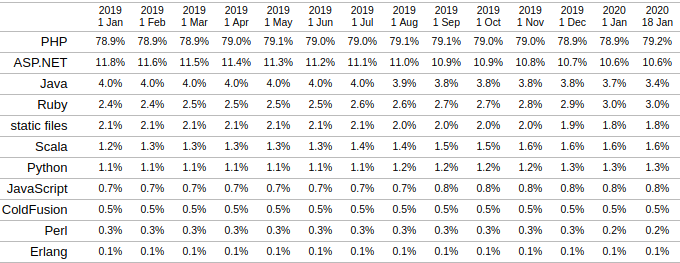
\includegraphics[width=6in]{images/php.png}
    \caption{Przedstawienie użycia języków po stronie serwera na podstawie strony https://w3techs.com/technologies/history\_overview/programming\_language na dzień 12.01.2020  \label{fig:php}}
\end{figure}